\documentclass[tikz,border=7pt]{standalone}
\usepackage[T1]{fontenc}
\usepackage{lmodern}
\usepackage{helvet}
\renewcommand{\familydefault}{\sfdefault}
\usepackage{amsmath}
\usepackage{xcolor}
\usepackage{tikz}
\usetikzlibrary{
  arrows.meta,
  positioning,
  calc,
  fit,
  shapes.geometric,
  shapes.symbols,
  backgrounds,
  decorations.pathreplacing,
  decorations.pathmorphing,
}

\definecolor{slate}{HTML}{334155}
\definecolor{teal}{HTML}{0D9488}
\definecolor{amber}{HTML}{D97706}
\definecolor{rose}{HTML}{E11D48}
\definecolor{muted}{HTML}{64748B}
\definecolor{line}{HTML}{94A3B8}
\definecolor{pagebg}{HTML}{F8FAFC}
\definecolor{card}{HTML}{FFFFFF}
\definecolor{lightteal}{HTML}{CCFBF1}
\definecolor{lightamber}{HTML}{FEF3C7}
\definecolor{lightrose}{HTML}{FFE4E6}
\definecolor{lightslate}{HTML}{E2E8F0}
\definecolor{blueink}{HTML}{2563EB}
\definecolor{bluewash}{HTML}{DBEAFE}
\definecolor{greenink}{HTML}{16A34A}
\definecolor{greenwash}{HTML}{DCFCE7}
\definecolor{pinkink}{HTML}{DB2777}
\definecolor{pinkwash}{HTML}{FCE7F3}

\tikzset{
  >=Stealth,
  font=\sffamily\scriptsize,
  every node/.append style={text=slate},
  title/.style={font=\sffamily\bfseries\small, text=slate, anchor=west},
  note/.style={font=\sffamily\tiny, text=muted, align=left},
  label/.style={font=\sffamily\tiny, text=muted},
  chip/.style={
    draw=#1,
    fill=#1!12,
    rounded corners=2pt,
    inner sep=2.5pt,
    font=\sffamily\tiny\bfseries,
    text=slate,
  },
  decision/.style={
    shape=diamond,
    aspect=2.1,
    draw=teal,
    fill=lightteal,
    inner sep=1.5pt,
    align=center,
    font=\sffamily\tiny,
    text=slate,
  },
  pics/person/.style 2 args={
    code={
      \fill[#1] (0,0.92) circle (0.18);
      \fill[#1]
        (-0.26,0.68)
        .. controls (-0.34,0.42) and (-0.30,0.18) .. (-0.22,0.02)
        -- (0.22,0.02)
        .. controls (0.30,0.18) and (0.34,0.42) .. (0.26,0.68)
        -- cycle;
      \node[font=\sffamily\tiny\bfseries, text=#1, anchor=north] at (0,-0.08) {#2};
    }
  },
  pics/disk/.style={
    code={
      \fill[lightslate] (0,-0.04) ellipse (0.28 and 0.10);
      \fill[slate] (-0.28,-0.04) rectangle (0.28,0.12);
      \fill[slate] (0,0.12) ellipse (0.28 and 0.10);
      \fill[card] (0,0.14) ellipse (0.11 and 0.04);
    }
  },
}

\begin{document}
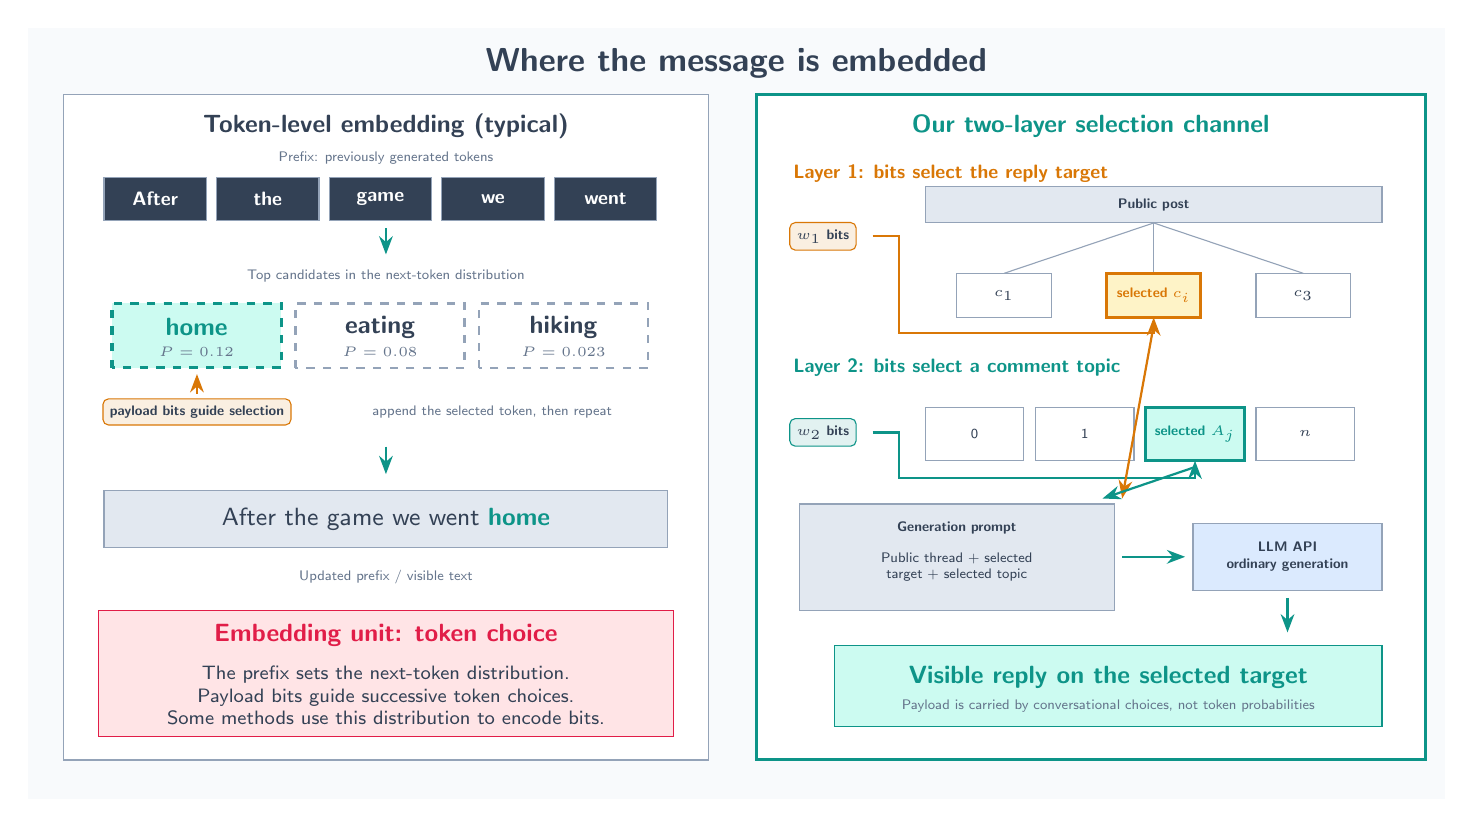
\begin{tikzpicture}[x=1cm,y=1cm]
  \fill[pagebg] (-0.25,-0.2) rectangle (17.75,9.6);
  \node[font=\sffamily\bfseries\large,text=slate] at (8.75,9.15)
    {Where the message is embedded};

  % Token-level baseline
  \fill[card] (0.2,0.3) rectangle (8.4,8.75);
  \draw[line] (0.2,0.3) rectangle (8.4,8.75);
  \node[font=\sffamily\bfseries\small,text=slate] at (4.3,8.35)
    {Token-level embedding (typical)};

  \node[label] at (4.3,7.95) {Prefix: previously generated tokens};
  \foreach \i/\tok in {0/After,1/the,2/game,3/we,4/went} {
    \pgfmathsetmacro{\xx}{0.72+\i*1.43}
    \fill[slate] (\xx,7.15) rectangle (\xx+1.30,7.70);
    \draw[line] (\xx,7.15) rectangle (\xx+1.30,7.70);
    \node[font=\sffamily\scriptsize\bfseries,text=card] at (\xx+0.65,7.425) {\tok};
  }
  \draw[teal,->,thick] (4.3,7.05) -- (4.3,6.72);
  \node[label] at (4.3,6.45) {Top candidates in the next-token distribution};

  % Candidate next tokens with their conditional probabilities.
  \foreach \x/\tok/\prob in {0.82/home/0.12,3.15/eating/0.08,5.48/hiking/0.023} {
    \fill[card] (\x,5.28) rectangle (\x+2.15,6.10);
    \draw[dashed,line width=0.9pt,line] (\x,5.28) rectangle (\x+2.15,6.10);
    \node[font=\sffamily\small\bfseries] at (\x+1.075,5.80) {\tok};
    \node[font=\sffamily\tiny,text=muted] at (\x+1.075,5.48) {$P=\prob$};
  }
  \fill[lightteal] (0.82,5.28) rectangle (2.97,6.10);
  \draw[teal,line width=1.2pt,dashed] (0.82,5.28) rectangle (2.97,6.10);
  \node[font=\sffamily\small\bfseries,text=teal] at (1.895,5.80) {home};
  \node[font=\sffamily\tiny,text=muted] at (1.895,5.48) {$P=0.12$};

  \node[chip=amber] at (1.90,4.72) {payload bits guide selection};
  \draw[amber,->,thick] (1.90,4.95) -- (1.90,5.20);
  \node[label] at (5.65,4.72) {append the selected token, then repeat};
  \draw[teal,->,thick] (4.3,4.28) -- (4.3,3.93);
  \fill[lightslate] (0.72,3.00) rectangle (7.88,3.72);
  \draw[line] (0.72,3.00) rectangle (7.88,3.72);
  \node[font=\sffamily\small,align=center] at (4.3,3.36)
    {After the game we went \textcolor{teal}{\bfseries home}};
  \node[label] at (4.3,2.62) {Updated prefix / visible text};

  \fill[lightrose] (0.65,0.60) rectangle (7.95,2.20);
  \draw[rose] (0.65,0.60) rectangle (7.95,2.20);
  \node[font=\sffamily\small\bfseries,text=rose] at (4.3,1.88)
    {Embedding unit: token choice};
  \node[font=\sffamily\scriptsize,text=slate,align=center,text width=6.8cm]
    at (4.3,1.12) {The prefix sets the next-token distribution.\\Payload bits guide successive token choices.\\Some methods use this distribution to encode bits.};

  % Two-layer selection-channel method
  \fill[card] (9.0,0.3) rectangle (17.5,8.75);
  \draw[teal,line width=1.1pt] (9.0,0.3) rectangle (17.5,8.75);
  \node[font=\sffamily\bfseries\small,text=teal] at (13.25,8.35)
    {Our two-layer selection channel};

  % Layer 1: choose a reply target in the shared thread.
  \node[font=\sffamily\scriptsize\bfseries,text=amber,anchor=west]
    at (9.35,7.75) {Layer 1: bits select the reply target};
  \node[chip=amber] at (9.85,6.95) {$w_1$ bits};
  \draw[amber,->,thick] (10.48,6.95) -- (10.82,6.95) -- (10.82,5.72) -- (14.05,5.72) -- (14.05,5.92);
  \fill[lightslate] (11.15,7.12) rectangle (16.95,7.58);
  \draw[line] (11.15,7.12) rectangle (16.95,7.58);
  \node[font=\sffamily\tiny\bfseries] at (14.05,7.35) {Public post};
  \draw[line] (14.05,7.12) -- (12.15,6.48);
  \draw[line] (14.05,7.12) -- (14.05,6.48);
  \draw[line] (14.05,7.12) -- (15.95,6.48);
  \fill[card] (11.55,5.92) rectangle (12.75,6.48);
  \draw[line] (11.55,5.92) rectangle (12.75,6.48);
  \node[font=\sffamily\tiny] at (12.15,6.20) {$c_1$};
  \fill[lightamber] (13.45,5.92) rectangle (14.65,6.48);
  \draw[amber,line width=1.1pt] (13.45,5.92) rectangle (14.65,6.48);
  \node[font=\sffamily\tiny\bfseries,text=amber] at (14.05,6.20) {selected $c_i$};
  \fill[card] (15.35,5.92) rectangle (16.55,6.48);
  \draw[line] (15.35,5.92) rectangle (16.55,6.48);
  \node[font=\sffamily\tiny] at (15.95,6.20) {$c_3$};

  % Layer 2: choose a comment topic from the shared list.
  \node[font=\sffamily\scriptsize\bfseries,text=teal,anchor=west]
    at (9.35,5.28) {Layer 2: bits select a comment topic};
  \node[chip=teal] at (9.85,4.46) {$w_2$ bits};
  \draw[teal,->,thick] (10.48,4.46) -- (10.82,4.46) -- (10.82,3.88) -- (14.575,3.88) -- (14.575,4.10);
  \foreach \x/\lab in {11.15/0,12.55/1,13.95/$k$,15.35/$n$} {
    \fill[card] (\x,4.10) rectangle (\x+1.25,4.78);
    \draw[line] (\x,4.10) rectangle (\x+1.25,4.78);
    \node[font=\sffamily\tiny] at (\x+0.625,4.44) {\lab};
  }
  \fill[lightteal] (13.95,4.10) rectangle (15.20,4.78);
  \draw[teal,line width=1.1pt] (13.95,4.10) rectangle (15.20,4.78);
    \node[font=\sffamily\tiny\bfseries,text=teal] at (14.575,4.44) {selected $A_j$};

  % Synthesis from public context and the two selected choices.
  \fill[lightslate] (9.55,2.20) rectangle (13.55,3.55);
  \draw[line] (9.55,2.20) rectangle (13.55,3.55);
  \node[font=\sffamily\tiny\bfseries] at (11.55,3.25) {Generation prompt};
  \node[font=\sffamily\tiny,align=center,text width=3.5cm]
    at (11.55,2.75) {Public thread + selected target + selected topic};
  \draw[amber,->,thick] (14.05,5.82) -- (13.65,3.62);
  \draw[teal,->,thick] (14.575,4.02) -- (13.40,3.62);

  \fill[bluewash] (14.55,2.45) rectangle (16.95,3.30);
  \draw[line] (14.55,2.45) rectangle (16.95,3.30);
  \node[font=\sffamily\tiny\bfseries,align=center] at (15.75,2.88)
    {LLM API\\ordinary generation};
  \draw[teal,->,thick] (13.65,2.88) -- (14.45,2.88);
  \draw[teal,->,thick] (15.75,2.36) -- (15.75,1.92);

  \fill[lightteal] (10.0,0.72) rectangle (16.95,1.75);
  \draw[teal] (10.0,0.72) rectangle (16.95,1.75);
  \node[font=\sffamily\small\bfseries,text=teal] at (13.475,1.35)
    {Visible reply on the selected target};
  \node[label] at (13.475,0.98) {Payload is carried by conversational choices, not token probabilities};
\end{tikzpicture}
\end{document}
